\section{The LHC coordinate system}
\label{s:lhc_cord}
Most of the detectors placed at the IRs have a cylindrical shape with the axis of
the cylinder lying along the beam direction. Within the detectors, various sub-detectors are placed
either parallel (barrel region) to the beam direction or perpendicular (endcap region) to it.
At the LHC, the $z$-axis lies along the beam direction, while the $x$-$y$ plane is perpendicular 
to it as shown in Figure~\ref{fig:lhc_cord}. 
%https://wiki.physik.uzh.ch/cms/latex:example_spherical_coordinates
\begin{figure}
  \begin{center}
  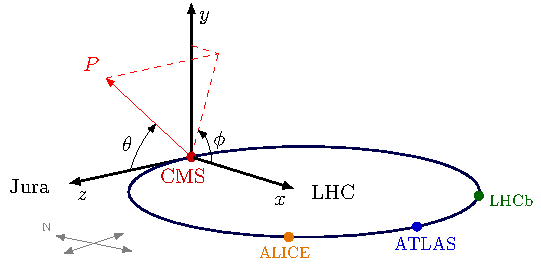
\includegraphics[width=0.50\linewidth]{Experiment/LHC/Image/cord.pdf}
  \caption{The LHC coordinate system \cite{CMSWiki} with the $z$-axis lying along the beam direction. 
	At CMS, the $z$-axis points towards the mountain Jura in France.}
  \label{fig:lhc_cord}
  \end{center}
\end{figure}
The following derived quantities are often used by the LHC experiments:
\begin{itemize}[leftmargin=*]
\item $\textbf{Transverse momentum (\pt)}$: 
	Out of $10^{11}$ protons in a bunch, only about 20 hard collisions occur 
	in one bunch crossing. Rest of the protons move in the forward region, some of 
	them with soft collision and some even without being collided. The hard 
	collisions produce actual physics process of interest. Due to the head-on 
	collision, the particles produced in hard collisions mostly go in the transverse 
	plane. The momentum in the $x$-$y$ plane, \pt, is defined as
	\begin{equation}
		\pt = \sqrt{p_x^2 + p_y^2}
	\end{equation}
	where $p_x$ and $p_y$ are the $x$ and $y$ components of the momentum vector, respectively. 
	Detecting a higher \pt in an event indicates the occurrence of actual physics process.
\item $\textbf{Pseudorapidity $(\eta)$}$: As shown in Figure~\ref{fig:lhc_cord}, 
	the azimuthal angle ($\phi$) is the angle between $\vec{p_x}$ and the $x$-axis. 
	It covers the full barrel region and ranges from 0 to 2$\pi$. On the other hand $\theta$ 
	is the angle between the momentum vector $\vec{p}$ and $z$-axis which varies from 0 to 
	$\pi$ to cover both sides of the endcap. 
	In the collider experiments, one measures 4-vector ($E, \vec{p}$) of a 
	particle. Just looking at the 4-vector, its not easy to predict the direction
	of the particle with respect to the beam axis. In view of this, there is a quantity 
	called \dq{rapidity}, given by \cite{EDaw}
	\begin{equation}
		y = \frac{1}{2}\ln\left(\frac{E+p_z}{E-p_z}\right)
	\label{eq:lhc_y}
	\end{equation}
	which is very useful to know the value of $\theta$. For example, $y = 0$ implies 
	that $E > p_z$. That is, the particle is produced in the transverse plane which
	implies $\theta = \pi/2$. For $y = \pm 1$, $E<p_z$. That is the particle is
	moving mostly in the beam direction implying $\theta = 0$ or $\pi$. The
	another advantage of rapidity is that the difference in rapidities is Lorentz 
	invariant. For example, under the Lorentz boost, the 4-momentum transforms as 
	$E^\prime = \gamma (E-\beta p_z) , ~p^\prime_x = p_x, ~p^\prime_y = p_y, ~p^\prime_z = \gamma(p_z - \beta E)$, so the rapidity is transformed as
	\begin{equation}
		y^\prime = y - \tanh^{-1}\beta
	\end{equation}
	where $\beta = v$ ($v$ is the velocity of the boosted frame), and 
	$\gamma = \sqrt{1-\beta^2}$. If an observer measures rapidities of two particles
	in the boosted frame then difference $y_1^\prime -y_2^\prime = y_1 - y_2$.
	That is, the difference in rapidities is Lorentz invariant. This is very useful
	when one is interested in the angular separation between two physics objects such
	as a muon and a hadronic jet.

	The relativistic limit of rapidity is called pseudorapidity ($\eta$). In such limit, 
	the momentum of a particle is much larger than its rest mass 
	, that is, $E = \sqrt{p^2 + m_0^2} \approx p$. Therefore, Equation (\ref{eq:lhc_y}) becomes
	\begin{equation}
		y = - \ln\tan \left(\frac{\theta}{2}\right) \to \eta
	\label{lhc_eta}
	\end{equation}
	The $\eta$ variable is mostly used everywhere at the LHC as it is directly related to the
	angle $\theta$. The relationship between $\eta$ and $\theta$ is shown in Figure 
	\ref{fig:lhc_eta}.
	%https://en.wikipedia.org/wiki/Pseudorapidity
	\begin{figure}
	\begin{center}
	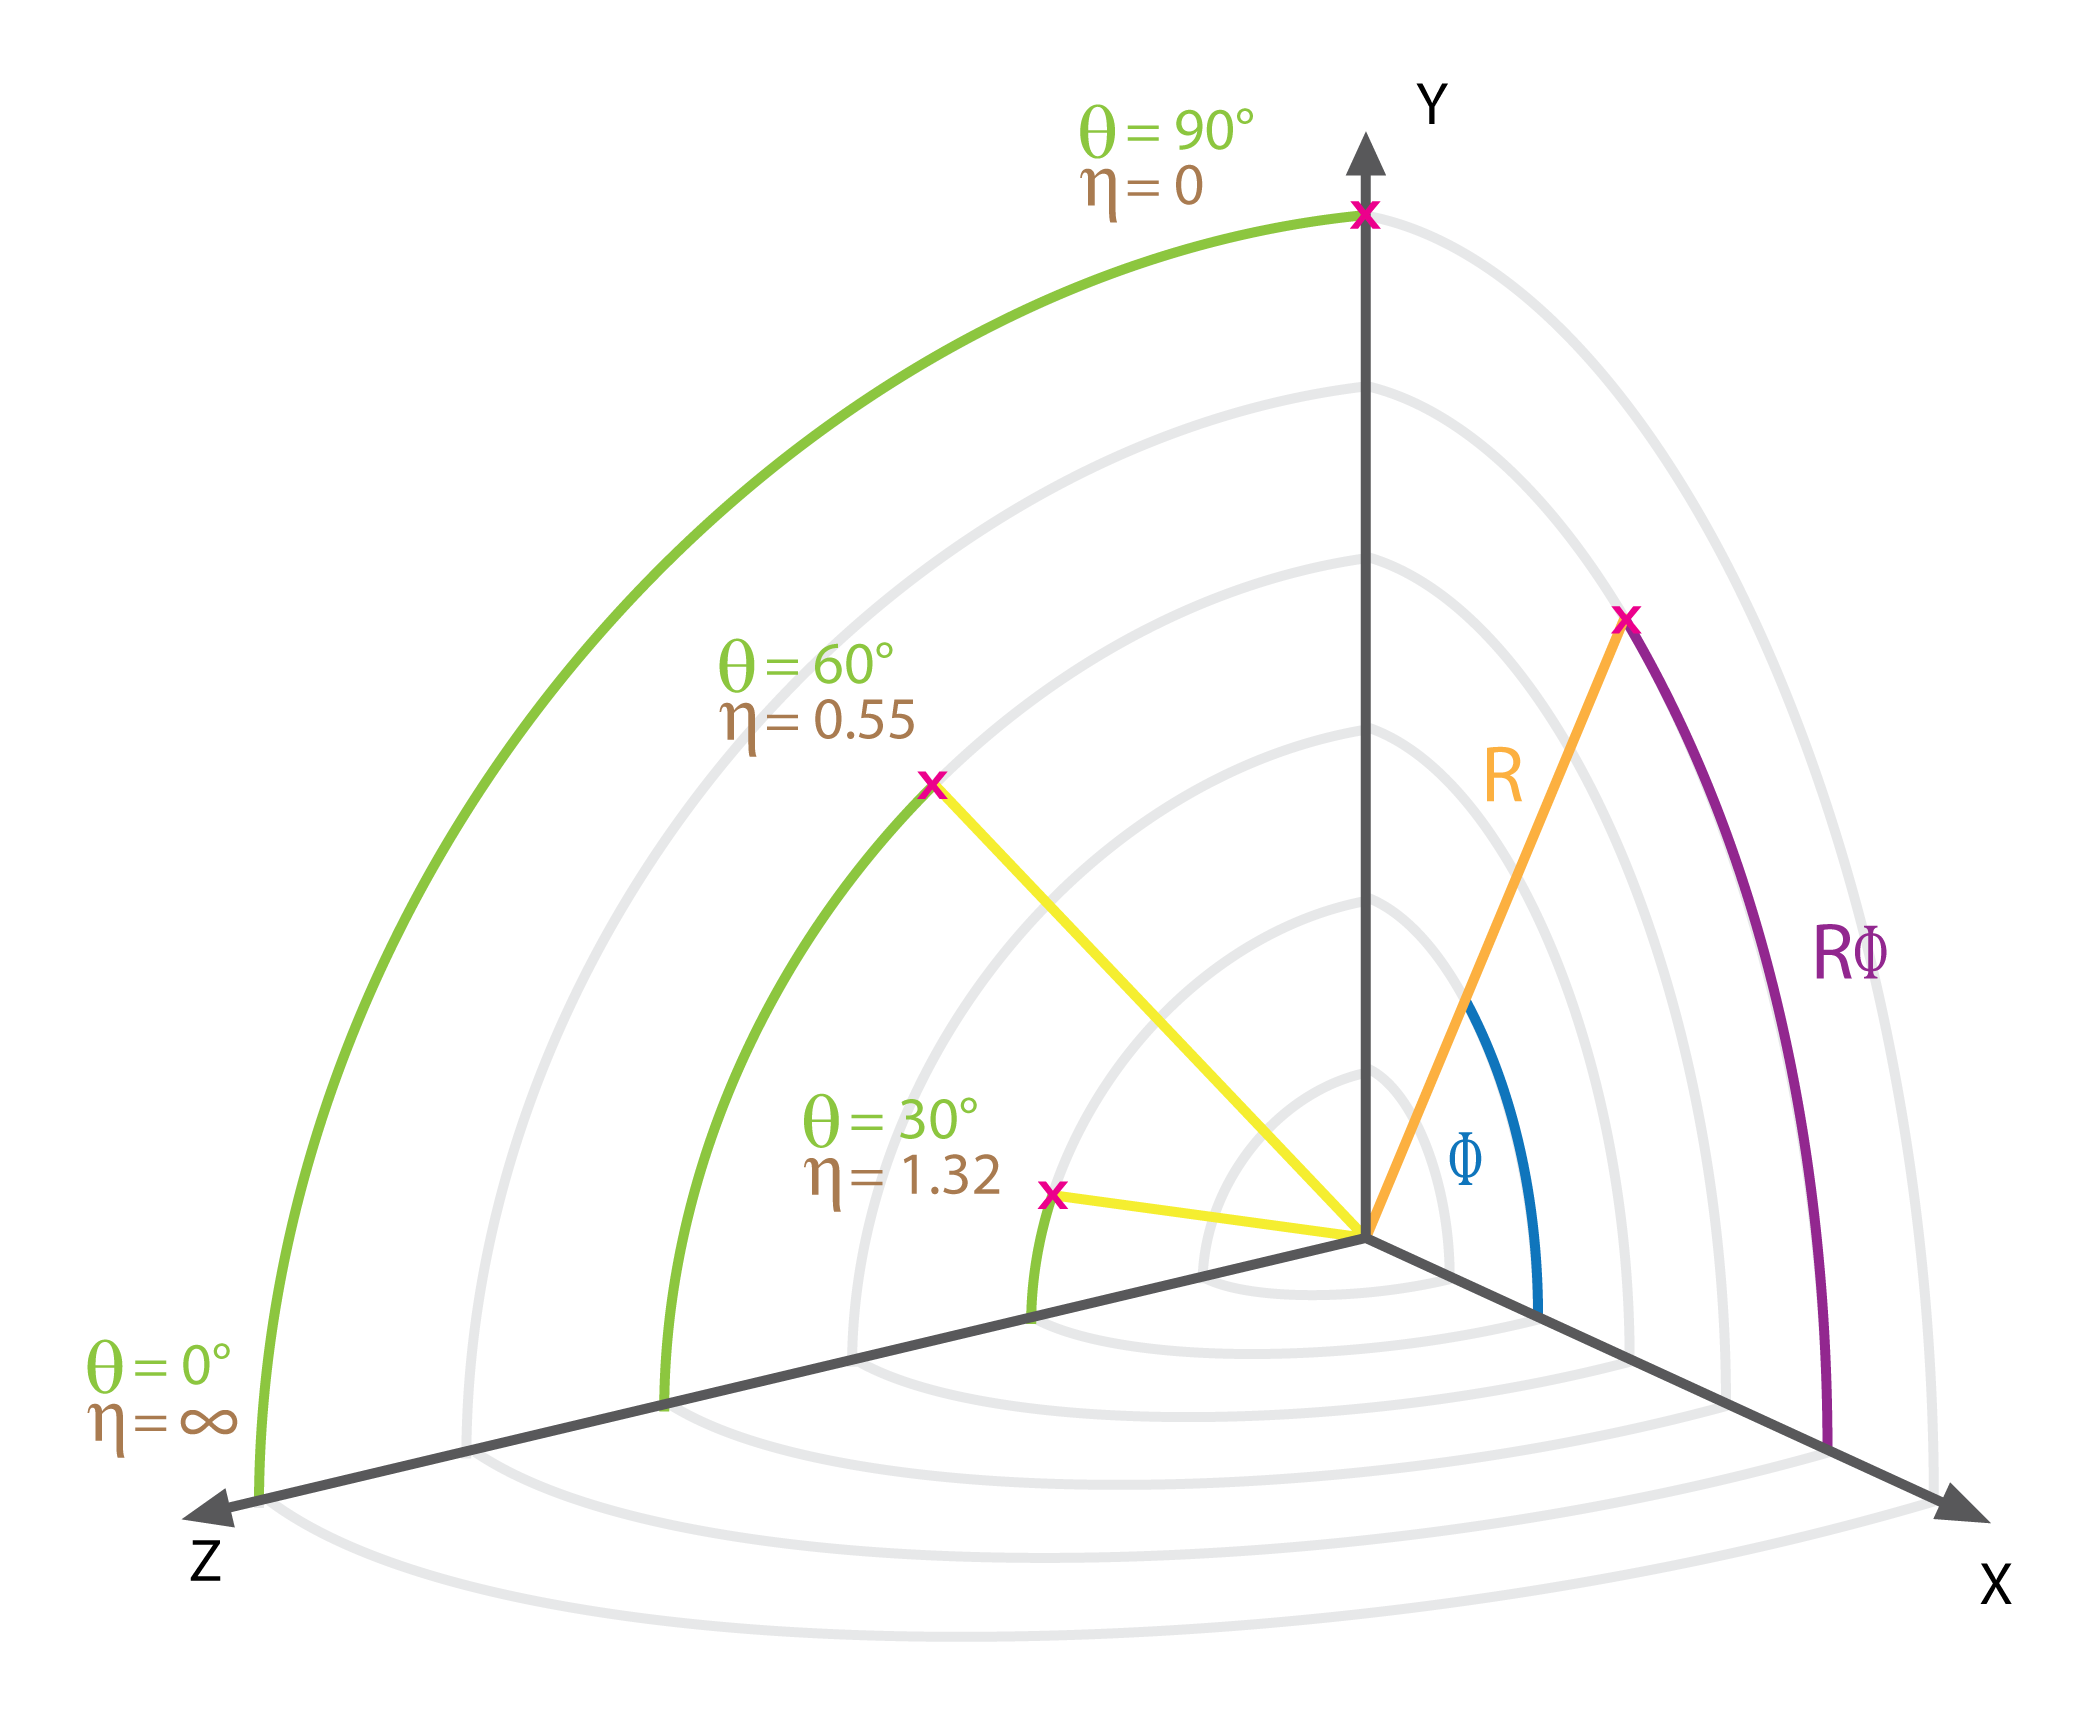
\includegraphics[width=0.50\linewidth]{Experiment/LHC/Image/lhc_eta.png}
		\caption{The relationship between $\theta$ and $\eta$ \cite{Lenzi:2013xpa}. The 
	value of $\eta = 0$ implies $\theta = \pi/2$. That is, lower the value of $\eta$ the farther 
	away we are from the beam axis in the perpendicular direction and vice versa.}
	\label{fig:lhc_eta}
	\end{center}
	\end{figure}
	One can see that for a large value of $\eta$, \eg, $\eta = 4 (-4)$, the particle is 
	close to the beam axis [$\theta = 0 (\pi)$]. Similarly, the lower value of $\eta$ indicates 
	that the particle is produced in the transverse plane. The lower and higher values of
	$\eta$ correspond to barrel and endcap region of the detector, respectively.
\end{itemize}
